\begin{figure}[h]
  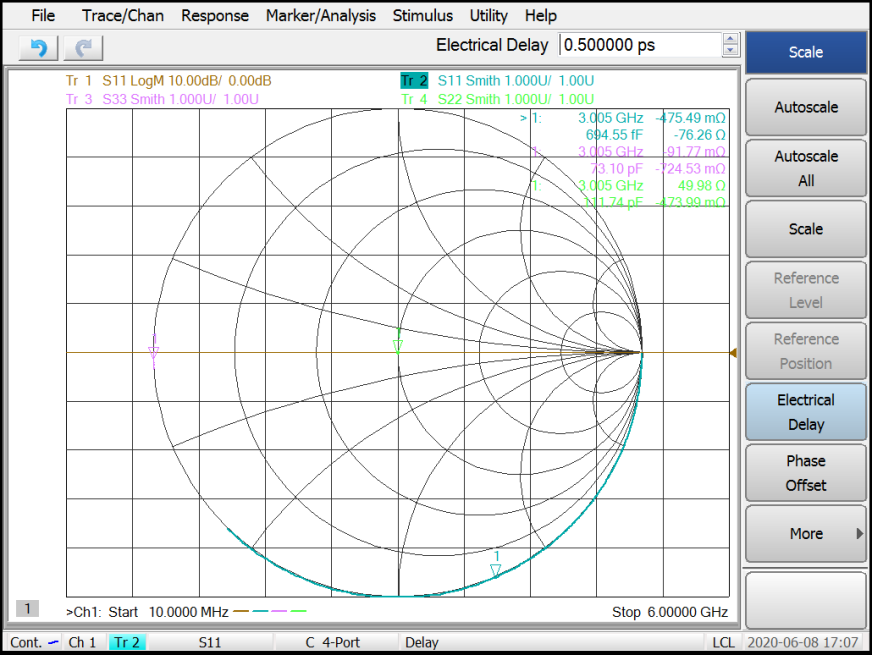
\includegraphics[width=\textwidth]{2_3_2}
  \caption{Smithdiagramm der S11-Messung, im Trace 2 ist ein Kapazitiver anteil
    bei offenem Abschluss erkennbar}
  \label{fig:2_3_2}
\end{figure}

\begin{figure}[h]
  \begin{center}
  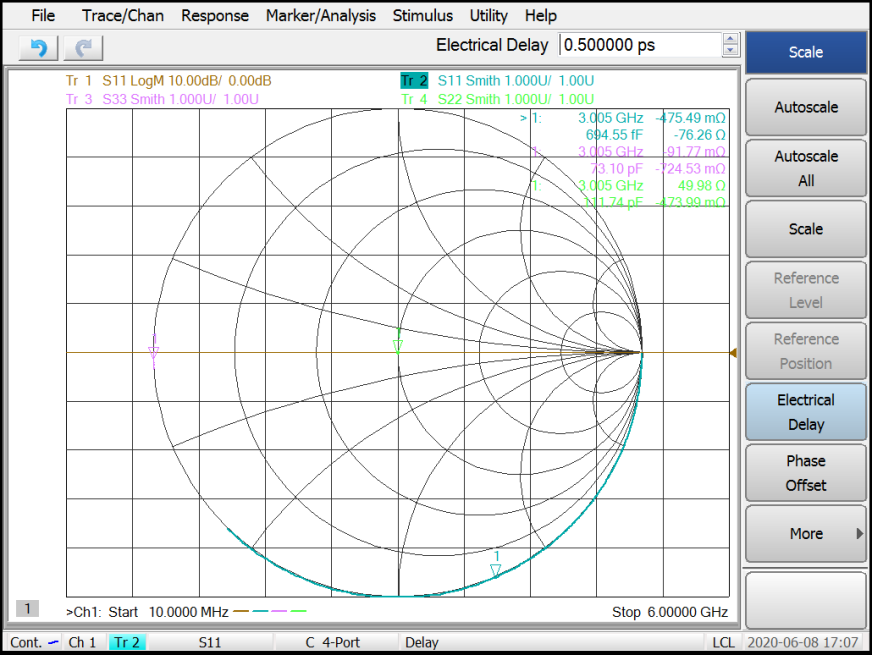
\includegraphics[width=0.618\textwidth]{2_3_2}
  \caption{Smithdiagramm der S11-Messung, mit Korrekturparameter, Türkis: Open,
    Grün: Load, Pink: Short}
  \label{fig:2_3_1}
  \end{center}
\end{figure}

\begin{figure}[h]
  \begin{center}
  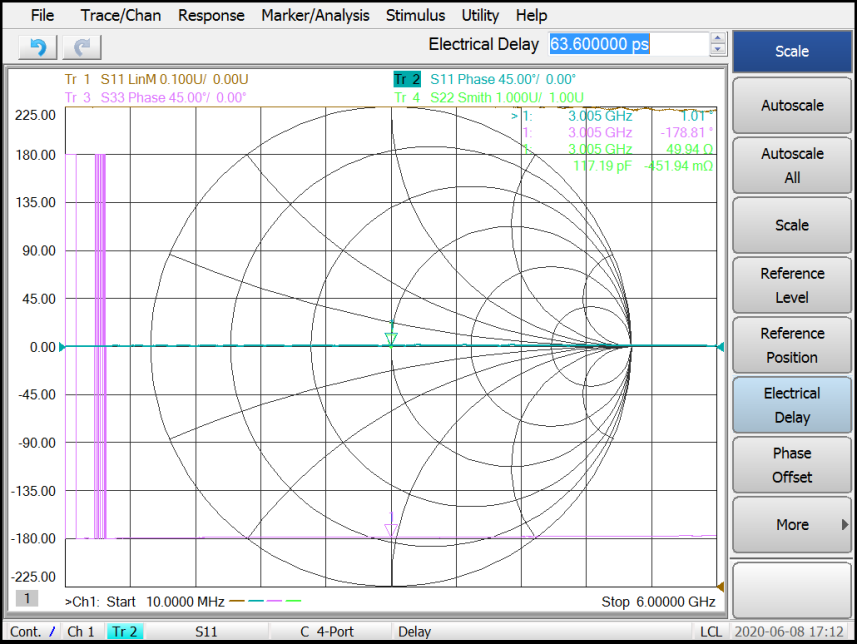
\includegraphics[width=0.618\textwidth]{phase}
  \caption{Phasen der S11-Messung, Farben entsprechen Abb. \ref{fig:2_3_1}}
  \label{fig:phase_2_3}
  \end{center}
\end{figure}

Mithilfe eines mechanischen Standards wurde das DUT, ein Koaxialkabel,
jeweils mit Short, Open und Load abgeschlossen und der S11-Parameter mit dem
Netzwerkanalysator als Frequenzgang bestimmt. Vorher musste noch der kapazitive
Anteil des S11 mithilfe eines \emph{Electrical Delays} in der Software des
Netzwerkanalysators kompensiert werden (Abb. \ref{fig:2_3_2}).

Daraufhin wurde
die S11-Parameter Leitung bei den entsprechenden Abschlüssen gemessen und unter
Umständen mit einem Electrical Delay beaufschlagt. Im Ergebniss erkennt man die
S11-Positionen im Smithdiagramm bei Short am linken Rand mit Phase $-180 \, \si{\degree}$ (0 auf der reelen
Achse), also Totalreflexion, bei Open am rechten Rand mit Phase $0 \, \si{\degree}$ ($\infty$ auf der reelen
Achse), auch Totalreflexion, und bei Load in der Mitte ($1$ auf der reelen
Achse). Das Smithdiagramm zeigt die erwarteten Ergebnisse (Abb. \ref{fig:2_3_1}).

Über der Frequenz
waren die Reflexionsfaktoren bei Short sowie Open entsprechend $0 \,
\si{\deci\bel}$ und bei Load (Anpassung) bei einem sehr geringen Wert, was
ebenfalls zu erwarten war.
